\documentclass[10pt,letterpaper]{article}

\usepackage[T1]{fontenc}
\usepackage[utf8]{inputenc}
\usepackage{lmodern}
% Times for text, Helvetica for sans serif, Computer Modern for mathematics
% and code: the single-column preprint layout of NeurIPS-style papers.
\renewcommand{\rmdefault}{ptm}
\usepackage[scaled=0.92]{helvet}
\usepackage{microtype}
\DisableLigatures[-]{encoding=T1,family=tt*}
\usepackage[letterpaper,textwidth=5.5in,textheight=9in,top=1in,hcentering]{geometry}
\usepackage{titlesec}
\usepackage{amsmath,amssymb,amsthm}
\usepackage{booktabs}
\usepackage{enumitem}
\usepackage{xcolor}
\usepackage{listings}
% Palette: one primary colour, one accent and neutrals. All pass contrast
% on white and stay distinct in grayscale and for common colour blindness.
\definecolor{kitprimary}{HTML}{0B4F8A}
\definecolor{kitaccent}{HTML}{B5470F}
\definecolor{kitmuted}{HTML}{5F6B7A}
\definecolor{kittint}{HTML}{EEF3F9}
\usepackage{float}
\usepackage{fancyvrb}
\usepackage{upquote}
\usepackage{tikz}
\usetikzlibrary{arrows.meta}
\usepackage[numbers,sort&compress]{natbib}
\usepackage[colorlinks,linkcolor=kitprimary,citecolor=kitprimary,urlcolor=kitprimary]{hyperref}
\usepackage[capitalise,noabbrev]{cleveref}

\setlist{nosep}
\setlength{\parindent}{0pt}
\setlength{\parskip}{5.5pt plus 1pt minus 1pt}
\titleformat*{\section}{\large\bfseries\color{kitprimary}}
\titleformat*{\subsection}{\normalsize\bfseries\color{kitprimary}}
\titlespacing*{\section}{0pt}{12pt plus 4pt minus 2pt}{6pt plus 2pt}
\titlespacing*{\subsection}{0pt}{9pt plus 3pt minus 2pt}{4pt plus 1pt}
\renewenvironment{abstract}
  {\begin{center}\large\bfseries Abstract\end{center}\vspace{-1ex}%
   \list{}{\leftmargin=0.5in\rightmargin=0.5in}\item\relax}
  {\endlist}
\setlength{\textfloatsep}{12pt plus 2pt minus 4pt}
\setlength{\emergencystretch}{3em}

% Code: pseudocode for the algorithms, shell for the appendix.
\lstdefinelanguage{kitpseudo}{
  morekeywords={if,for,each,in,while,return,require,reject,continue,and,or,not,is,
    last,enumerate},
  morecomment=[l]{\#},
  morestring=[b]",
  sensitive=true,
}
\lstdefinestyle{kitcode}{
  basicstyle=\ttfamily\scriptsize,
  keywordstyle=\bfseries\color{kitprimary},
  commentstyle=\itshape\color{kitmuted},
  stringstyle=\color{kitaccent},
  backgroundcolor=\color{kittint},
  columns=fullflexible, keepspaces=true, showstringspaces=false,
  upquote=true, frame=none, aboveskip=2pt, belowskip=0pt,
  xleftmargin=4pt, framexleftmargin=4pt,
}
\lstdefinestyle{kitalgo}{style=kitcode, language=kitpseudo,
  numbers=left, numberstyle=\tiny\color{kitmuted}, numbersep=6pt,
  xleftmargin=16pt}
\lstdefinestyle{kitshell}{style=kitcode, language=bash, morekeywords={cargo,git,python3},
  keywordstyle=\color{kitprimary}}

% Pseudocode floats in plain verbatim style.
\floatstyle{ruled}
\newfloat{algorithm}{tbp}{loa}
\floatname{algorithm}{Algorithm}
\crefname{algorithm}{Algorithm}{Algorithms}

\newtheorem{definition}{Definition}
\newtheorem{lemma}{Lemma}
\newtheorem{proposition}{Proposition}
\theoremstyle{remark}
\newtheorem{remark}{Remark}
\crefname{definition}{Definition}{Definitions}
\crefname{lemma}{Lemma}{Lemmas}
\crefname{proposition}{Proposition}{Propositions}

\newcommand{\kit}{\textsf{kit}}
\newcommand{\Hb}{\mathsf{H}}
\newcommand{\D}{\mathsf{D}}
\newcommand{\BMT}{\mathsf{BMT}}
\newcommand{\cc}{\mathbin{\|}}
\newcommand{\str}[1]{\texttt{"\romannumeral-`0#1"}}
\newcommand{\bytes}[1]{\texttt{\romannumeral-`0#1}}
\newcommand{\sha}{96fb9ee9afdb890f74a639c3419a402d205cfa71}
\newcommand{\repo}[1]{\href{https://github.com/officialunofficial/kit/blob/\sha/#1}{\expandafter\nolinkurl\expandafter{\romannumeral-`0#1}}}

\hypersetup{
  pdftitle={kit: An Offline-Verifiable Repository},
  pdfauthor={Christopher Wallace, Vitor Marthendal, Erica Gregor},
}

\begin{document}

\begin{center}
  \rule{\textwidth}{4pt}\par\vspace{0.25in}
  {\LARGE\bfseries \kit: An Offline-Verifiable Repository\par}
  \vspace{0.29in}\rule{\textwidth}{1pt}\par\vspace{0.3in}
  \begin{tabular}{@{}c@{\hspace{2.5em}}c@{\hspace{2.5em}}c@{}}
    \textbf{Christopher Wallace}\textsuperscript{$*$} &
    \textbf{Vitor Marthendal} &
    \textbf{Erica Gregor} \\
    Official Unofficial, Inc. & Official Unofficial, Inc. & Official Unofficial, Inc.
  \end{tabular}\par\vspace{0.3in}
\end{center}

{\renewcommand{\thefootnote}{}%
 \footnotetext{\textsuperscript{$*$}Corresponding author:
   \href{mailto:christopher@officialunofficial.com}{\texttt{christopher@officialunofficial.com}}.}%
 \footnotetext{Preprint. Version 0.1 (draft), 30 October 2026. This work is
   licensed under the Creative Commons Attribution 4.0 International License
   (CC~BY~4.0).}}


\begin{abstract}
A version-control client usually trusts the server, forge and mirrors that hand
it bytes. \kit{} is a content-addressed, signed version-control system that
removes that trust for claims about content. It names every object with a hash
shaped like the proof a verifier needs: trees and chunk lists by typed binary
Merkle roots, blobs by their BLAKE3 hash, which is also their Bao root, and a
commit by a hash that covers its mandatory Ed25519 signature. From one trusted
commit id, a verifier can check offline that a path, a chunk or a byte range
belongs to the commit, and that a served object set holds every object the
commit reaches. Each verifier returns what it authenticated rather than what it
was told. A disclosure bundle grows with path depth and with the logarithm of
directory size and chunk count, not with repository size, and an absolute file
offset costs no more at the last chunk than at the first: in our committed vectors a file
at depth 3 (two directories below the root) costs 635 bytes, 318 of them the
bundle header, commit id and signed commit, and each further directory of $M$
entries adds about $75 + |\mathit{name}| + 32\lceil\log_2 M\rceil$ bytes. We
give the construction, the two verifiers, and informal security arguments that
reduce soundness to BLAKE3 collision resistance. \kit{} is alpha software
(version 0.5.0), and the disclosure format is a draft specification.
\end{abstract}

% ---------------------------------------------------------------------------
\section{Introduction}\label{sec:intro}

A developer who clones a repository trusts the host that serves it. If the
host swaps a file, drops a commit or serves a stale tree, most clients do not
notice, because the identifiers they hold do not cover enough. In git, commit
signing is optional and object ids are SHA-1 by default~\cite{git}. A git tree
id commits to the full entry list of a directory, so a proof that one file
belongs to a commit carries every directory listing on its path, and a check
that a mirror served all of a commit's objects requires a full fetch and walk.

\kit{} asks one question of every format: what can a verifier check, offline,
from a single commit id $c^\star$ it already trusts? A \kit{} verifier can
check, with no network access and no trust in the party that served the bytes,
that the commit carries a valid signature, that a path, a chunk or a byte range
is part of $c^\star$, and that a set of served objects contains every object
$c^\star$ reaches. With a user-chosen list of trusted keys it can also check
who signed. The verifier must still obtain $c^\star$ from a source it trusts,
such as a release note, a signed tag or a colleague. After that, the server,
the forge and every mirror are untrusted for these claims.

\kit{} names every object with a hash shaped like the proof a verifier needs.
Trees and chunk lists are named by typed binary Merkle roots, blobs by their
BLAKE3 hash, which is also their Bao root, and a commit by a hash that covers
its signature. One trusted commit id is then enough for a verifier to check
offline that a path, a chunk or a byte range is in the commit, and that a
served object set is complete. One principle shapes both verifiers:
\emph{untrusted metadata is a hint; only recomputed hashes are evidence.} Each
verifier returns what it authenticated, not what the prover claimed or the
caller asked for. The rule runs through the paper: a disclosure reports the
authenticated path, a closure manifest only locates packs, closure keys objects
by recomputed id, and the directory an attestation is stored under is not
evidence.

\paragraph{Who receives a proof.}
An auditor or licence checker who needs one file, a reproducible-build system
that needs pinned inputs, a partial mirror, and a verifier running in a browser
all want to check a claim about part of a commit without cloning it or
trusting the host. For example, a build service fetches \texttt{src/lib.rs}
from an untrusted mirror together with a bundle, checks the bundle against the
release's commit id, and gets the authenticated path and bytes. It never
downloads the rest of the repository.

\paragraph{What is new.}
Merkle inclusion proofs are textbook~\cite{merkle1987,rfc6962}; the question is
what a repository's ids must look like for such proofs to reach from a commit
to a byte. A git tree hashes the full listing, so a path proof carries every
listing on the path. A single authenticated dictionary over all paths, such as
a sparse Merkle tree or a Merkle Patricia trie~\cite{smt,ethereum}, gives
logarithmic proofs but makes a commit commit to one global structure, so
unchanged subdirectories are no longer objects shared between commits. IPFS
UnixFS~\cite{unixfs} shards large directories with a HAMT, so proof size
depends on the sharding. What \kit{} adds is the combination: per-directory,
typed binary Merkle ids that keep git's subtree sharing; blob ids that are Bao
roots, so byte ranges need no extra commitment; a mandatory signature inside
the commit id; and a completeness verdict that needs no repository.

\paragraph{Contributions.}
\begin{itemize}
  \item \emph{Proof-shaped identifiers} (\cref{sec:objects}). The combination
        above: trees and chunked files are named by a binary Merkle root that
        binds the leaf count, wrapped in a type domain, and flat objects by
        BLAKE3 over canonical bytes, so a blob id is its Bao root. One trusted
        commit id then authenticates a path, a chunk or a byte range through
        objects that commits already share.
  \item \emph{Disclosure as a hash chain from $c^\star$}
        (\cref{sec:disclosure}). Each step is checked against the id the step
        above authenticated. A chunk leaf commits the chunk's byte span, so one
        proof of a chunk gives its absolute file offset without disclosing
        earlier chunks. The verifier returns the path, leaf id and offsets it
        proved. Bundle size grows with path depth times the logarithm of
        directory width, plus the logarithm of the chunk count, plus the
        payload. It does not grow with repository size or with the chunk
        index.
  \item \emph{Closure as an offline completeness verdict}
        (\cref{sec:closure}). The verifier keys every supplied object by its
        recomputed id, walks from the caller's root, and reports missing,
        corrupt and unreferenced objects. ``Complete'' means every reachable
        object is present and is the one the root determines, under collision
        resistance alone, with no local repository.
  \item Security arguments for these claims under BLAKE3 collision resistance
        (\cref{sec:security}), and proof sizes measured from committed vectors
        (\cref{sec:eval}).
\end{itemize}

\paragraph{Paper structure.}
\Cref{sec:model} sets out the threat model and goals, \cref{sec:objects} the
identifiers, \cref{sec:disclosure,sec:closure} the two verifiers and
\cref{sec:signing} signatures. \Cref{sec:security,sec:eval} give the security
arguments and measurements, and \cref{sec:related,sec:limits,sec:conclusion}
cover related work, limitations and conclusions. \Cref{app:repro} holds
reference material and the commands that reproduce each result.

% ---------------------------------------------------------------------------
\section{Setting, threat model and goals}\label{sec:model}

\paragraph{Parties.}
An \emph{author} holds an Ed25519 signing seed and creates commits, remixes and
tags. A \emph{verifier} checks a claim about content. An \emph{untrusted
server} is any party that stores or forwards bytes: a forge, a mirror, an
object-store bucket or a network peer. The adversary controls every untrusted
server and chooses every byte the verifier receives, including refs, packs,
bundles, manifests and attestation envelopes. It can generate keys and sign its
own commits.

\paragraph{Trust inputs.}
The verifier trusts one commit id $c^\star$ (or a remix or tag id) obtained out
of band. For claims about \emph{who} signed, it also trusts a list of keys that
the user maintains. The list comes from the user's configuration; a file inside
the repository is refused unless the user names it explicitly, so a hostile
clone cannot plant keys. \Cref{tab:inputs}
shows what each check needs.

\begin{table}[t]
\centering\small
\caption{Inputs that each check needs. ``Bytes'' are untrusted bytes from any
source. No check needs a local repository.}\label{tab:inputs}
\begin{tabular}{@{}lccc@{}}
\toprule
Check & Commit id & Bytes & Trusted keys \\
\midrule
Signature valid under embedded key & \checkmark & \checkmark & \\
Disclosure of a path, chunk or range & \checkmark & \checkmark & \\
Closure completeness & \checkmark & \checkmark & \\
Signer is trusted & \checkmark & \checkmark & \checkmark \\
Attestation about the commit & \checkmark & \checkmark & \checkmark \\
\bottomrule
\end{tabular}
\end{table}

\paragraph{Assumptions.}
\begin{description}[leftmargin=1.5em]
  \item[A1 (hash).] BLAKE3~\cite{blake3} is collision resistant. Range proofs
        use Bao slices~\cite{bao}, which expose BLAKE3's internal chaining
        values, so A1 also covers collisions of those values.
  \item[A2 (signature).] Ed25519~\cite{ed25519,rfc8032} is EUF-CMA secure
        under the acceptance predicate of SPEC-SIGNING: canonical
        encodings of $A$ and $R$, neither of small order, $0 \le S < L$, and
        the cofactored equation $[8]([S]B - R - [k]A) = 0$~\cite{taming}.
        Single and batch checks use the same cofactored equation, so they
        agree on every signature~\cite{taming}.
  \item[A3 (implementation).] The verifier implements its specification.
        Byte-exact golden vectors pass both the Rust code and an independent
        reference written from the specifications, and every decoder and
        verifier on these paths has a fuzz target; \cref{app:assurance}
        summarizes this evidence, which does not prove A3.
  \item[A4 (host).] The verifier's host and every process with the user's UID
        are trusted.
\end{description}
\kit{} signs a BLAKE3 digest, not the raw signing bytes, so the unforgeability
of a commit signature rests on A1 and A2 together.

\paragraph{Out of scope.}
The meaning of an attestation predicate; trusted time, since timestamps are
self-reported; the host and every process with the user's UID; and recovery
from key compromise, since there is no in-band revocation.
\emph{Availability}: a server can refuse to serve, and the verifier detects a
mismatch with $c^\star$ but cannot force delivery. \emph{Freshness}: whether
$c^\star$ is the latest commit of a branch is a property of the channel that
delivered it. A valid signature binds a commit to a key, not to a person.

\paragraph{Goals.}
A prover holding the repository wants to convince a verifier that holds only
$c^\star$ of one of two statements: ``$x$ is the content at path $p$ (and
offset $o$) of $c^\star$'', or ``set $O$ contains the full closure of
$c^\star$''. We want \emph{soundness}: an accepted statement is true of the
state that $c^\star$ determines, unless the adversary found a BLAKE3 collision
(\cref{sec:security}). The \emph{depth} $d$ of a path is its number of
components, so \texttt{src/lib.rs} has depth 2 and a disclosure carries one
step per component. We want \emph{succinctness}: a disclosure for depth $d$,
directory widths $M_1, \dots, M_d$, $K$ chunks and a range of $\ell$ bytes
costs $O(\sum_j \log M_j + \log K + \ell)$ hashes, independent of repository
size. We want a \emph{bounded verifier}: no prover-supplied length sizes an
allocation before it is checked against a fixed cap.

% ---------------------------------------------------------------------------
\section{Proof-shaped identifiers}\label{sec:objects}

\paragraph{Notation.}
$\Hb(x)$ is BLAKE3 in default mode with a 32-byte output, $x \cc y$ is
concatenation, $\mathrm{le}_k$ and $\mathrm{be}_k$ are $k$-bit little- and
big-endian encodings, and $|x|$ is a length in bytes. Object ids and signing
digests use one domain-separation function:
\begin{equation}\label{eq:dd}
  \D(d, x) \;=\; \Hb\bigl(\mathrm{le}_{16}(|d|) \cc d \cc x\bigr).
\end{equation}

\paragraph{Canonical encoding.}
Every object starts with a type byte and a fixed magic and version. Integers
are fixed-width and every variable-length field carries its length. Readers
reject unknown types or versions, trailing bytes, unsorted or repeated tree
entries, and invalid entry names, and bound every count before allocation
(\cref{app:bounds}). Each accepted object therefore has exactly one encoding
(\cref{lem:inj}), and the store recomputes the id on every read. This section
follows SPEC-OBJECTS and SPEC-MERKLE-OBJECTS.

\paragraph{Flat and Merkle ids.}
Commits, remixes, tags and blobs are \emph{flat}; trees and chunked blobs are
\emph{Merkle} objects. A \emph{remix} is a signed commit-like object that names
a tree and cites commits from other repositories as sources, without including
them; a verifier treats it as a commit whose sources are references only.

\begin{definition}[Flat id]\label{def:flat}
For a flat object $o$ with canonical bytes $\beta(o)$,
$\mathrm{id}(o) = \Hb(\beta(o))$. A blob with data $x$ has
$\mathrm{id} = \Hb(\bytes{0x01} \cc \str{KOB1} \cc \bytes{0x01} \cc
\mathrm{le}_{32}(|x|) \cc x)$, and the id of a commit covers every field of the
commit, the signature included.
\end{definition}

\paragraph{A blob id is its Bao root.}
Because a flat id is BLAKE3 over the canonical bytes, the id of a blob is
exactly the root that Bao~\cite{bao} computes over those bytes. A Bao slice
that verifies against the blob id therefore authenticates a byte range
directly, and content offset $o$ is Bao offset $o + 10$ (the six-byte prologue
and four-byte length). Range proofs need no structure beyond the id the parent
tree already holds.

\begin{definition}[Binary Merkle tree]\label{def:bmt}
For leaf digests $L_0, \dots, L_{N-1}$, level~0 holds
$n^0_i = \Hb(\mathrm{be}_{32}(i) \cc L_i)$, or the single node
$\Hb(\varepsilon)$ if $N = 0$. Each higher level pairs adjacent nodes as
$\Hb(\mathit{left} \cc \mathit{right})$; an odd last node pairs with itself.
Folding ends at one node $t$, and
$\BMT(L_0, \dots, L_{N-1}) = \Hb(\mathrm{be}_{32}(N) \cc t)$.\footnote{This
tree and its proof encoding match an existing open-source BMT
implementation~\cite{commonware}.}
\end{definition}

\begin{definition}[Tree id]\label{def:tree}
A tree with entries $(\mathit{name}_i, \mathit{mode}_i, h_i)_{i<M}$ in
canonical order has leaves
$L_i = \D\bigl(\str{kit-tree-entry-v1},\, \mathrm{le}_{32}(|\mathit{name}_i|)
\cc \mathit{name}_i \cc \mathit{mode}_i \cc h_i\bigr)$ and id
$\mathrm{id}(T) = \D\bigl(\str{kit.tree\textbackslash 0},\, \BMT(L_0, \dots,
L_{M-1})\bigr)$.
\end{definition}

\begin{definition}[Chunked-blob id]\label{def:chunked}
A chunked blob with total size $s$, chunk-size field $z$ and chunks
$(c_i, e_i)_{i<K}$, where $c_i$ is the id of chunk $i$ and $e_i$ the end of its
byte span, with $e_{-1} = 0$ and span $[e_{i-1}, e_i)$, has leaves
$L_0 = \D(\str{kit-cblob-meta-v2}, \mathrm{le}_{64}(s) \cc \mathrm{le}_{32}(z))$
and $L_{i+1} = \D(\str{kit-cblob-chunk-v1}, \mathrm{le}_{64}(e_{i-1}) \cc
\mathrm{le}_{64}(e_i) \cc c_i)$, and id $\mathrm{id}(B) =
\D\bigl(\str{kit.chunked\textbackslash 0},\, \BMT(L_0, \dots, L_K)\bigr)$.
Chunk $i$ sits at position $i+1$. The stored manifest is $22 + 40K$ bytes, one
40-byte entry per chunk (an id and an end).
\end{definition}

\paragraph{What the wrap and the count prevent.}
The \emph{inner root} of a Merkle object is its $\BMT$ value before the outer
wrap. (i) Binding $N$ rules out the classic odd-node duplication
malleability, in which a sequence whose last node is repeated folds to the same
top node as the shorter sequence; it is defense in depth alongside the position
hashed into each level-0 node. (ii)
Without the outer type wrap, an empty tree and an empty chunked blob, or a
one-entry tree and a one-chunk blob over the same child, could share an id, so
a verifier that compared a proof with a bare inner root could accept a tree as
a chunked file. (iii) The metadata leaf binds the total size $s$ and the
chunk-size field $z$, which the chunk list does not determine, and each chunk
leaf binds the chunk's span with its id, so one proof of a chunk gives its place
in the file and its committed length. The length
prefix in a tree leaf stops $(\str{ab}, m, h)$ and $(\str{a}, m, \str{b} \cc
h')$ from aliasing. Every domain tag and magic is unique and never changes
(\cref{app:tags}).

\begin{figure}[!htb]
\centering
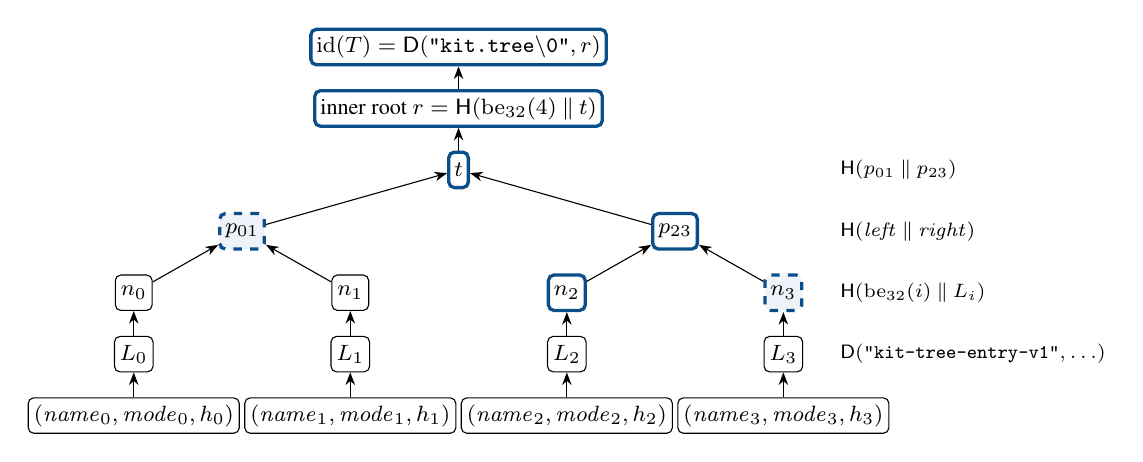
\begin{tikzpicture}[
  every node/.style={font=\footnotesize},
  nd/.style={draw, rounded corners=2pt, minimum height=4.5mm, inner sep=2pt},
  pth/.style={nd, very thick, draw=kitprimary},
  sib/.style={nd, fill=kittint, dashed, very thick, draw=kitprimary},
  ar/.style={-{Stealth[length=1.6mm]}}]
  \def\dx{2.75}\def\dy{0.78}
  \foreach \i in {0,1,2,3} {
    \node[nd] (e\i) at (\i*\dx,0) {$(\mathit{name}_\i, \mathit{mode}_\i, h_\i)$};
    \node[nd] (l\i) at (\i*\dx,\dy) {$L_\i$};
    \draw[ar] (e\i) -- (l\i);
  }
  \node[nd]  (n0) at (0,2*\dy) {$n_0$};
  \node[nd]  (n1) at (\dx,2*\dy) {$n_1$};
  \node[pth] (n2) at (2*\dx,2*\dy) {$n_2$};
  \node[sib] (n3) at (3*\dx,2*\dy) {$n_3$};
  \foreach \i in {0,1,2,3} { \draw[ar] (l\i) -- (n\i); }
  \node[sib] (p01) at (0.5*\dx,3*\dy) {$p_{01}$};
  \node[pth] (p23) at (2.5*\dx,3*\dy) {$p_{23}$};
  \draw[ar] (n0) -- (p01); \draw[ar] (n1) -- (p01);
  \draw[ar] (n2) -- (p23); \draw[ar] (n3) -- (p23);
  \node[pth] (t) at (1.5*\dx,4*\dy) {$t$};
  \draw[ar] (p01) -- (t); \draw[ar] (p23) -- (t);
  \node[pth] (r) at (1.5*\dx,5*\dy) {inner root $r = \Hb(\mathrm{be}_{32}(4) \cc t)$};
  \draw[ar] (t) -- (r);
  \node[pth] (id) at (1.5*\dx,6*\dy) {$\mathrm{id}(T) = \D(\str{kit.tree\textbackslash 0}, r)$};
  \draw[ar] (r) -- (id);
  \foreach \y/\t in {1/{$\D(\str{kit-tree-entry-v1}, \ldots)$},
                     2/{$\Hb(\mathrm{be}_{32}(i) \cc L_i)$},
                     3/{$\Hb(\mathit{left} \cc \mathit{right})$},
                     4/{$\Hb(p_{01} \cc p_{23})$}}
    \node[anchor=west, font=\scriptsize] at (3*\dx+0.6,\y*\dy) {\t};
\end{tikzpicture}
\caption{A four-entry tree id. The proof that entry~2 belongs to
$\mathrm{id}(T)$ carries the shaded siblings $n_3$ and $p_{01}$ in level-major
order. The verifier recomputes the thick nodes, wraps $r$ and compares the
result with the id it trusts, never with a bare $r$.}
\label{fig:tree}
\end{figure}

\paragraph{Inclusion proofs.}
A proof is the leaf count $N$ and the sibling digests on the path from the
leaf, bottom-up, omitting a sibling when a node pairs with itself. A
\emph{multi-proof} for a set of positions takes the positions in sorted order
and carries the siblings their paths need, level by level from the bottom, in
ascending position order within a level; a sibling that another path in the
set already computes is omitted, and each sibling is consumed once. The decoder
bounds the sibling count before reading any. The verifier folds the leaves to
an inner root, wraps it with the type domain, and compares the result with the
trusted id, never with a bare inner root. It rejects a position $\ge N$, a
repeated position, and a chunk proof at the metadata position. \Cref{fig:tree}
shows one proof.

\paragraph{Chunked files.}
Files over 1~MiB are split by FastCDC~\cite{fastcdc} (average chunk 64~KiB;
SPEC-FASTCDC). Each chunk is a blob whose id is a leaf of
\cref{def:chunked}, so a chunk proof is an inclusion proof and a range inside a
chunk is a Bao slice against the chunk id. Conformant chunkers agree on
boundaries, but readers also accept other valid layouts of the same bytes, so
the same file can have more than one id (\cref{sec:limits}).

\paragraph{Design space.}
For a path through directories of widths $M_1, \dots, M_d$, a git path proof
carries $\sum_j M_j$ entries. A global sparse Merkle tree or Merkle Patricia
trie over $n$ paths carries $O(\log n)$ digests and also supports absence
proofs, and an IPFS HAMT carries a number that depends on the sharding. \kit{}
keeps one object per directory and puts a binary Merkle tree inside it, so a
proof carries $\sum_j \lceil\log_2 M_j\rceil$ siblings (\cref{sec:eval}
measures both on real repositories).

% ---------------------------------------------------------------------------
\section{Verifiable disclosure}\label{sec:disclosure}

A disclosure bundle proves that one path, chunk or byte range belongs to a
commit. The verifier takes a trusted commit id and the bundle and nothing
else. It proves inclusion only: not that nothing else exists under a
directory, and not who holds the signing key. This section and the next follow
SPEC-DISCLOSURE, which is a draft specification of alpha software (\kit{}
0.5.0).

\paragraph{Bundle.}
A bundle holds the commit id, the commit bytes, one \emph{step} per path
component (root first), and a payload. A step carries the
entry's name, mode and child id, the parent tree's inner root, the entry's
position, and a single-leaf proof. The payload is the leaf object's canonical
bytes (\emph{Object}), one chunk with its span and a proof over the metadata leaf
and the chunk's leaf (\emph{Chunk}), or a Bao slice against the blob or chunk id
(\emph{Range}). A range inside a chunk carries the same chunk header, so its
absolute offset is the span start plus the offset in the chunk.

\begin{figure}[!htb]
\centering
\resizebox{\linewidth}{!}{%
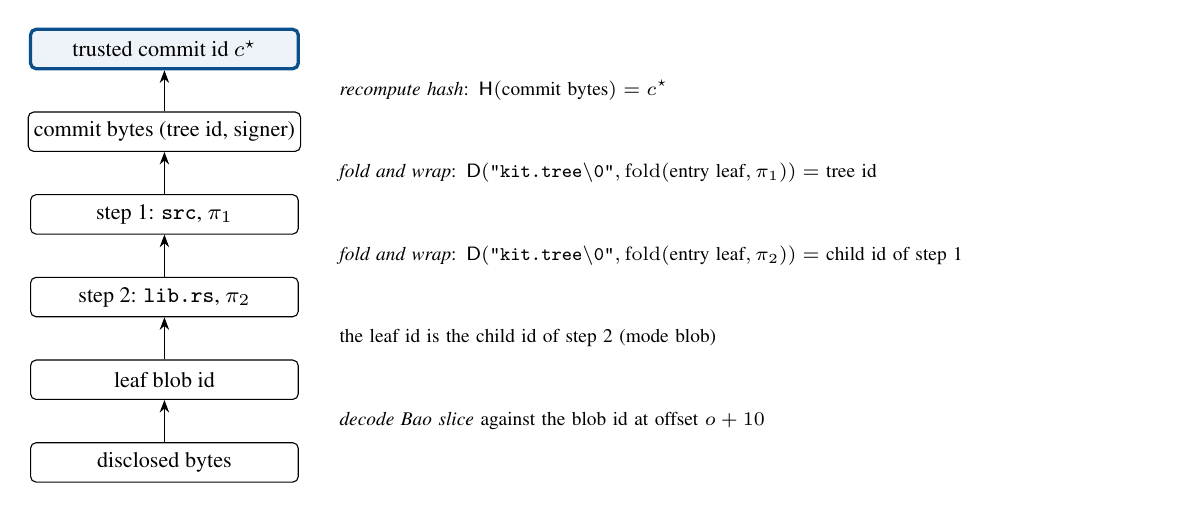
\begin{tikzpicture}[
  every node/.style={font=\footnotesize},
  box/.style={draw, rounded corners=2pt, minimum height=5mm, inner sep=2pt, align=center, minimum width=3.4cm},
  ar/.style={-{Stealth[length=1.6mm]}},
  lab/.style={font=\scriptsize, align=left, anchor=west, text width=10.4cm}]
  \def\dy{1.05}
  \node[box, very thick, draw=kitprimary, fill=kittint] (c) at (0,0) {trusted commit id $c^\star$};
  \node[box] (cb) at (0,-1*\dy) {commit bytes (tree id, signer)};
  \node[box] (s1) at (0,-2*\dy) {step 1: \texttt{src}, $\pi_1$};
  \node[box] (s2) at (0,-3*\dy) {step 2: \texttt{lib.rs}, $\pi_2$};
  \node[box] (bl) at (0,-4*\dy) {leaf blob id};
  \node[box] (pl) at (0,-5*\dy) {disclosed bytes};
  \draw[ar] (cb) -- (c);  \draw[ar] (s1) -- (cb); \draw[ar] (s2) -- (s1);
  \draw[ar] (bl) -- (s2); \draw[ar] (pl) -- (bl);
  \node[lab] at (2.1,-0.5*\dy) {\emph{recompute hash}: $\Hb(\text{commit bytes}) = c^\star$};
  \node[lab] at (2.1,-1.5*\dy) {\emph{fold and wrap}: $\D(\str{kit.tree\textbackslash 0}, \mathrm{fold}(\text{entry leaf}, \pi_1)) =$ tree id};
  \node[lab] at (2.1,-2.5*\dy) {\emph{fold and wrap}: $\D(\str{kit.tree\textbackslash 0}, \mathrm{fold}(\text{entry leaf}, \pi_2)) =$ child id of step 1};
  \node[lab] at (2.1,-3.5*\dy) {the leaf id is the child id of step 2 (mode blob)};
  \node[lab] at (2.1,-4.5*\dy) {\emph{decode Bao slice} against the blob id at offset $o+10$};
\end{tikzpicture}}
\caption{Disclosure verification chain for a byte range of \texttt{src/lib.rs}.
Each arrow binds the lower value to the upper one, which is already
authenticated. The chain ends at $c^\star$, the only trusted input. The output
is the authenticated path $[(\texttt{src}, \text{tree}), (\texttt{lib.rs},
\text{blob})]$, the leaf id and the bytes.}
\label{fig:chain}
\end{figure}

\paragraph{Verification algorithm.}
\Cref{alg:disclosure} restates the verification requirements of the
specification, and \cref{fig:chain} shows the chain it checks. Size is checked
before decoding, and the hash that binds everything to the caller's input,
$\Hb(\text{commit bytes}) = c^\star$, before any structure is interpreted. At
each step the verifier recomputes the entry leaf, folds it with the proof,
wraps the result in the tree domain, and compares it with the id the step above
authenticated, never with an independently supplied root. The bundle carries
the parent's inner root only as a hint, which the verifier checks against the
same expected id.

\begin{algorithm}[!htb]
\caption{Disclosure verification. $B_{\max}$ and $d_{\max}$ are the bundle and
step caps of \cref{tab:bounds}.}\label{alg:disclosure}
\begin{lstlisting}[style=kitalgo]
VerifyDisclosure(c*, B):
  if |B| > B_max: reject                      # before any decode
  check header; decode body; bound every Vec before allocation; reject trailing bytes
  if H(B.commit_bytes) != c*: reject          # the binding step
  obj := strict_decode(B.commit_bytes); require obj is Commit or Remix
  expected := obj.tree_hash; if len(B.steps) > d_max: reject
  for i, s in enumerate(B.steps):
    validate_name(s.name)
    leaf := D("kit-tree-entry-v1", le32(|s.name|) || s.name || s.mode || s.child_id)
    if D("kit.tree\0", fold(leaf, s.position, s.proof)) != expected: reject
    if i is not last and s.mode != Tree: reject
    expected := s.child_id
  path := [(s.name, s.mode) for s in B.steps]; leaf_id := expected
  Object: id_of(strict_decode(bytes)) == leaf_id
  Chunk:  meta := D("kit-cblob-meta-v2", le64(total) || le32(cs))  # computed here
          leaf := D("kit-cblob-chunk-v1", le64(start) || le64(end) || H(bytes))
          D("kit.chunked\0", fold({0: meta, i+1: leaf}, proof)) == leaf_id
          span rules; |bytes| as a blob == end - start
  Range:  len > 0; [chunk header: as Chunk, with chunk_id in place of H(bytes)]
          o + len <= end - start; Bao slice at offset o+10, length len,
          against blob or chunk id; absolute offset := start + o
  return (path, leaf_id, payload, offsets, signer, signature_valid)
\end{lstlisting}
\end{algorithm}

\paragraph{Bounds before allocation.}
A hostile prover controls every length field. None sizes an allocation before
it is checked against a fixed cap, and a proof's leaf count is compared, never
used to allocate. The whole-bundle cap is checked before any decoding.
\Cref{app:bounds} lists the caps.

\paragraph{Return what was proved.}
The verifier never trusts a path, offset, position or length from the prover.
It returns what it authenticated: the path as (name, mode) pairs, the leaf id,
the offset, the chunk index and span, and the absolute offset. The caller compares these with its request. A bundle
that discloses \texttt{README.md} when the caller asked for
\texttt{secrets.env} verifies, and it is the caller that must notice the
different path. \Cref{prop:disclosure} is stated over these returned values.
The result also reports the signer and whether the signature is valid under
the embedded key. The library reports an invalid signature; it does not reject
the bundle, which leaves signer policy to the caller.

\paragraph{Absolute offsets and their cost.}
A Bao slice proves bytes at an offset inside one blob. A chunk leaf commits the
chunk's span $[\mathit{start}, \mathit{end})$, so the same multi-proof that
places the chunk gives the absolute offset, $\mathit{start}$ plus the offset in
the chunk, and no proof for an earlier chunk is needed. The cost is the
16-byte span in the chunk header, and it does not depend on the chunk index. The
verifier applies the span rules of the specification: a span is non-empty and
inside the file, the first chunk starts at 0, the last ends at the total size,
and a fixed-size layout follows its formula. A disclosure proves the committed
span, not that the manifest is well formed or that each span equals the length
of its chunk. A \emph{Chunk} payload is checked against its span, and a
\emph{Range} only lies inside it. Closure verification and store admission
check that spans equal real lengths.

\paragraph{Ranges across chunks.}
A range across chunk boundaries is proved by a container of whole-chunk bundles
with consecutive indices. It needs no anchor: each bundle proves its own span,
consecutive spans must meet, and the range must lie inside the first and last
spans.

% ---------------------------------------------------------------------------
\section{Closure verification}\label{sec:closure}

Disclosure answers ``is this in the commit?''; a closure answers ``did you send
all of it?'' The verifier takes a trusted root id (a
commit, remix or tag) and a sequence of untrusted object byte strings, and
checks that every object reachable from the root is present and re-hashes
to its id. This is close to git's connectivity check and to how any Merkle-DAG
client walks a graph, and it is not succinct: the verifier receives every
object. What it adds is a standalone verdict with a precise meaning, computed
over untrusted storage with no local repository.

\paragraph{Modes.}
$\mathrm{children}(o, m)$ defines what an object references in mode $m$. A
commit or remix references its tree, and its parents only in \emph{history}
mode; a tree its entries; a chunked blob its chunks; a tag its target.
\emph{Snapshot} mode, the default, covers the root and its tree closure;
history mode adds every ancestor and its tree. A remix's sources are never
followed: they are citations of commits in other repositories, not part of the
state the root names, so following them would make completeness depend on
objects outside the commit.

\paragraph{Untrusted framing.}
In practice the objects arrive in raw, uncompressed packs located by an
untrusted manifest; the manifest is a hint, and the verifier takes the root
from its caller and rejects a manifest that names another root.

\paragraph{Outcomes.}
The report lists \emph{missing} ids (reached, but no bytes supplied),
\emph{corrupt} bytes (they do not deserialize, and are keyed by their BLAKE3
hash) and \emph{unreferenced} objects (they deserialize but are never reached,
and are reported when the supplied set can be enumerated). The closure is
complete when \emph{missing} and \emph{corrupt} are empty. Extras are allowed
because a provider may serve a superset. Because objects are keyed by
recomputed id, a bit-flipped object that still deserializes is a different
object: it surfaces as \emph{missing} (the id the parent names) plus
\emph{unreferenced} (the id it now has), not as \emph{corrupt}. No server-given
name is ever trusted. \Cref{alg:closure} shows the walk.

\begin{algorithm}[!htb]
\caption{Closure verification over untrusted object bytes. $n_{\max}$ is the
object cap of \cref{tab:bounds}.}\label{alg:closure}
\begin{lstlisting}[style=kitalgo]
VerifyClosure(r*, m, objects):
  require |objects| <= n_max; M := {}; corrupt := []
  for each supplied byte string b:
    o := strict_decode(b) or (corrupt += H(b); continue)
    M[id_of(o)] := o                          # flat: H(b); Merkle: wrapped BMT root
  missing := []; seen := {r*}; queue := [r*]  # BFS from the trusted root only
  while queue: x := pop(queue)
    if x not in M: missing += x; continue
    for y in children(M[x], m): if y not in seen: seen += y; push(queue, y)
  unreferenced := keys(M) - seen
  return complete = (missing == [] and corrupt == []), missing, corrupt, unreferenced
\end{lstlisting}
\end{algorithm}

% ---------------------------------------------------------------------------
\section{Signatures}\label{sec:signing}

\paragraph{The signed digest.}
This section follows SPEC-SIGNING. A commit's \emph{signing bytes} are its
prologue, tree id, parent count and ids, author identity, length-prefixed
message, timestamp and signer key. The signer signs, with PureEdDSA, the
32-byte digest
\begin{equation}\label{eq:sig}
  \mu_{\text{commit}} = \D\bigl(\str{kit.commit\textbackslash 0},\;
  \mathit{signing\_bytes}\bigr).
\end{equation}
Remixes and tags use \str{kit.remix\textbackslash 0} and
\str{kit.tag\textbackslash 0}. The domains have lengths 11, 10 and 8, so the
length prefix alone separates them, and the strings also differ at byte~4. The
signature sits inside the commit id, so $c^\star$ authenticates it. The id also
covers two 32-byte annotation slots that lie outside the signature, so that
downstream annotations do not change what was signed. The consequence: anyone
holding a signed commit can change these slots and obtain a different commit
id whose signature still verifies. A signature therefore binds the signing
bytes, not one commit id. Disclosure and closure are unaffected, because they
bind to $c^\star$ itself, which fixes the slots.

\paragraph{Valid versus trusted.}
Verification rebuilds the signing bytes and applies the predicate of A2 with
the object's own key, so an adversary's self-signed commit passes. A separate
check looks the key up in the user's trusted keys and fails closed when it is
absent or the list is missing. The author field is an unauthenticated
attribution claim; a verifier must not treat a match between author and signer
key as evidence. Every commit is signed; the format has no unsigned variant.

\paragraph{Attestations.}
Claims about a commit are in-toto statements~\cite{intoto} in DSSE
envelopes~\cite{dsse} whose subject is the commit id. DSSE signs a
pre-authentication encoding (PAE) that starts with \str{DSSEv1} and carries the
payload type and payload with their lengths. The verifier decodes strictly and
rejects an envelope whose subject is not the commit being checked before it
checks any signature; the directory an envelope is stored under is not
evidence. A valid attestation shows that a trusted key signed a claim about the
commit, not that the claim is true.

% ---------------------------------------------------------------------------
\section{Security analysis}\label{sec:security}

The arguments below are informal and not machine-checked. They reduce a failure
to a BLAKE3 collision or an Ed25519 forgery. The author may be adversarial, so
the property is binding, not honesty. Under A1 and \cref{lem:inj}, $c^\star$
determines a unique commit object $C$ with $\Hb(\beta(C)) = c^\star$, and
through its tree id a unique state $S$. Soundness is the following experiment:
the adversary outputs $c^\star$ and a bundle (or object set), and wins if the
verifier accepts and its returned values differ from what $S$ determines. The
propositions bound the adversary's winning probability by the probability that
it finds a BLAKE3 collision.

\begin{lemma}[Encoding injectivity]\label{lem:inj}
Every hash input in \cref{eq:dd} and \cref{def:flat,def:bmt,def:tree,def:chunked}
is a fixed layout of fixed-width and length-prefixed fields, so distinct field
tuples give distinct inputs; and strict parsing gives each accepted object
exactly one encoding.
\end{lemma}
\begin{proof}[Sketch]
A length precedes each variable-length field and every other field has a fixed
width, so the bytes determine the fields. In \cref{eq:dd},
$\mathrm{le}_{16}(|d|) \cc d$ is self-delimiting. Rejecting trailing bytes,
unsorted or repeated entries and non-minimal varints leaves one encoding per
object.
\end{proof}

\begin{lemma}[BMT binding]\label{lem:bmt}
Under A1, no efficient adversary finds distinct leaf sequences with equal
$\BMT$ values. If a proof for position $p$ folds leaf $L$ to
$\BMT(L_0, \dots, L_{N-1})$, then $L = L_p$ unless a collision was found. If a
multi-proof for a position set $P$ folds leaves $(L'_p)_{p \in P}$ to that
value, then $L'_p = L_p$ for every $p \in P$ unless a collision was found.
\end{lemma}
\begin{proof}[Sketch]
$\Hb(\mathrm{be}_{32}(N) \cc t) = \Hb(\mathrm{be}_{32}(N') \cc t')$ with
distinct inputs is a collision, so $N = N'$ and $t = t'$, and $N$ fixes the
tree shape. Descending, equal parents give equal children or a collision; at
level~0, $\Hb(\mathrm{be}_{32}(i) \cc L_i) = \Hb(\mathrm{be}_{32}(i) \cc L'_i)$
gives $L_i = L'_i$ or a collision. For a proof, the verifier derives the path
from $(N, p)$, rejects $p \ge N$ and consumes each sibling once; the same
descent along the path gives $L = L_p$ or a collision. For a multi-proof, the
verifier derives every path from $(N, P)$ and each recomputed node lies on the
path of some $p \in P$; the descent along each path gives $L'_p = L_p$ or a
collision.
\end{proof}

\begin{proposition}[Disclosure binds bytes to the commit]\label{prop:disclosure}
Assume A1 and A3. If \cref{alg:disclosure} accepts $B$ against $c^\star$ and
returns path $\pi = [(n_1, m_1), \ldots, (n_k, m_k)]$, leaf id $\ell$ and bytes
$x$, then, unless a BLAKE3 collision was found, $S$ has a path
$n_1/\cdots/n_k$ with modes $m_1, \ldots, m_k$ ending at $\ell$, and $x$ is the
canonical bytes of $\ell$ (\emph{Object}); chunk $i$ of $\ell$, with the
returned total size and chunk-size field (\emph{Chunk}); or the content at the
returned offset and length of the blob $\ell$ or of its chunk $i$
(\emph{Range}). A returned absolute offset is the span start that the manifest
of $S$ commits to for chunk $i$, plus the offset of $x$ in the chunk.
\end{proposition}
\begin{proof}[Sketch]
Line~4 gives $\Hb(\text{commit bytes}) = \Hb(\beta(C))$, so the commit bytes
are $\beta(C)$, and the tree id, signer and signature are those of $C$. Induct
over steps with the invariant ``\emph{expected} is the id of the tree at
$n_1/\cdots/n_j$ in $S$''. The wrapped fold equals that id, so by
\cref{lem:inj} the fold equals the inner root of that tree in $S$, and by
\cref{lem:bmt} the recomputed leaf is the leaf of $S$ at $p_j$; \cref{lem:inj} on the leaf domain
makes $(n_j, m_j, \mathit{child}_j)$ the entry of $S$; the mode check keeps
every non-final child a tree. For \emph{Object}, $\mathrm{id}(x) = \ell$ pins
the flat bytes, or the Merkle leaves and so, by canonical encoding, the bytes.
For \emph{Chunk}, the wrapped multi-proof, whose metadata leaf and chunk leaf
the verifier computes itself, makes, by \cref{lem:bmt}, the total size, the
chunk-size field, the span and $\Hb(x)$, the chunk id, those of $S$. For \emph{Range},
the Bao root is $\Hb$ of the canonical bytes, and a slice that decodes to other
bytes gives a collision of BLAKE3 or its chaining values (A1). The chunk leaf pins
the span start, so the absolute offset is the start in $S$ plus the offset in
the chunk.
\end{proof}

\begin{remark}
\Cref{prop:disclosure} concerns the authenticated path, not the requested one.
It says nothing about absence, and its signature output states only validity
under the key in $C$. This is the formal form of ``return what was proved''.
\end{remark}

\begin{proposition}[A complete closure contains every reachable object]\label{prop:closure}
Assume A1 and A3. Let $R_m(r^\star)$ be the ids reachable from the root
$r^\star$ of $S$ under $\mathrm{children}(\cdot, m)$. If \cref{alg:closure}
reports \emph{complete}, then for every $x \in R_m(r^\star)$ the supplied set
holds an object $o$ with $\mathrm{id}(o) = x$, and $o$ is the object of $S$
with id $x$, unless a BLAKE3 collision was found.
\end{proposition}
\begin{proof}[Sketch]
$M$ keys each object by its recomputed id, never by a server-given name, and
the walk starts at the caller's $r^\star$, not at the manifest root. Induct on
breadth-first depth. Completeness means $M[r^\star]$ exists, and
$\mathrm{id}(M[r^\star]) = r^\star$ makes it the root object of $S$ or yields
a collision (\cref{lem:inj}; \cref{lem:bmt} for a Merkle type). If a visited
object is the object of $S$, $\mathrm{children}$, a deterministic function of
it, returns the children in $S$; each is in $M$, and then the object of $S$ by
the same argument, or reported missing. An empty \emph{missing} list therefore
means every $x \in R_m(r^\star)$ was found.
\end{proof}

The proposition covers what $\mathrm{children}$ follows: parents only in
history mode, never remix sources. It says nothing about the
signer or about whether the history is the latest.

\begin{proposition}[Signature non-replay across domains]\label{prop:replay}
Assume A1 and A2. An adversary that obtains signatures under an honest key
$\mathit{pk}$ on commits, remixes, tags and DSSE envelopes of its choice cannot
output an object or envelope that verifies under $\mathit{pk}$ in its own
domain unless $\mathit{pk}$ signed exactly that message, except with the
probability of an Ed25519 forgery or a BLAKE3 collision.
\end{proposition}
\begin{proof}[Sketch]
For the object domains, the signed message is
$\mu = \D(d_t, \mathit{signing\_bytes})$, and the hash inputs begin with
$\mathrm{le}_{16}(|d_t|) \cc d_t$ for lengths 11, 10 and 8, so inputs in
different domains differ before any adversary-chosen byte. Equal digests across
domains, or within one domain for different signing bytes (\cref{lem:inj}), are
a BLAKE3 collision. A DSSE message is a PAE string; the verifier requires the
28-byte payload type \texttt{application/vnd.in-toto+json}, so an accepted PAE
has at least $7 + 2 + 1 + 28 + 1 + 1 + 1 = 41$ bytes, while every object-domain
message has 32. These message sets are disjoint with no hash assumption. A
signature on a message $\mathit{pk}$ never signed is an Ed25519 forgery (A2).
The predicate rejects second encodings of $A$, $R$ and $S$, so a third party
cannot change the signature bytes of a signed commit and keep it
valid~\cite{taming}. It can change the annotation slots (\cref{sec:signing}),
which changes the id but not the signed message.
\end{proof}

The proposition does not cover a key also used for SSH or for other protocols,
whose messages \kit{} does not control.

% ---------------------------------------------------------------------------
\section{Evaluation}\label{sec:eval}

\paragraph{Proof size.}
A tree step costs the entry plus at most $32\lceil \log_2 M \rceil$ sibling
bytes for $M$ entries, a chunk step at most $32 \cdot 2\lceil \log_2 (K+1)
\rceil$ for $K$ chunks, and a Bao slice of $\ell$ content bytes about one
1~KiB block per KiB plus $64 \log_2(\text{blocks})$ bytes. For a 1~GiB file at
the 64~KiB average, $K \approx 16{,}384$, and the formula bounds a chunk step
at 30 siblings. Applying the sibling-selection rule of multi-proofs to
every chunk index gives an exact worst case of 27 (864 bytes), since the paths
from positions $0$ and $i+1$ meet by the top level and odd trailing nodes need
none. The same computation reproduces the sibling counts of \cref{tab:sizes}.
Proof size grows with path depth and the logarithm of directory size and chunk
count, not with repository size or with the chunk index.

\paragraph{Fixture.}
We measured the accepting disclosure vectors built on one fixture
(\cref{app:repro}). The fixture has a 279-byte signed commit, a 5-entry root
tree and a 1,048,577-byte file that FastCDC splits into 15 chunks.

\begin{table}[!htb]
\centering\footnotesize\setlength{\tabcolsep}{3pt}
\caption{Selected accepting disclosure vectors, in bytes (all eleven are in
\cref{tab:sizes-all}). ``Sibl.'' lists sibling digests per step. ``Payload''
is canonical object or chunk bytes, or a Bao slice; for a chunk or a chunk range the chunk proof has
the sibling count in parentheses. Every bundle also holds a
5-byte header, the 32-byte commit id and the 279-byte commit with a 2-byte
length.}
\label{tab:sizes}
\begin{tabular}{@{}lrrlrl@{}}
\toprule
Disclosure & Total & Steps & Sibl. & Payload & Kind (chunk proof) \\
\midrule
file at root                &    533 & 182 & 3       &     30 & object \\
file at depth 3 (two dirs)  &    635 & 272 & 1, 0, 0 &     42 & object \\
whole small blob as range   &  2,137 & 180 & 3       &  1,618 & range, 1,536 B \\
64 B in chunk 1             &  2,102 & 182 & 3       &  1,352 & range, 64 B (4 sibl.) \\
whole chunk 1               & 19,274 & 182 & 3       & 18,572 & chunk (4 sibl.) \\
\bottomrule
\end{tabular}
\end{table}

\paragraph{Results.}
\Cref{tab:sizes} shows that a whole small file costs 533 to 635 bytes (527 for
the smallest vector, \cref{tab:sizes-all}), of which 318 are the header,
commit id and commit. A step costs $75 + |\mathit{name}| + 32n$ bytes for $n$
siblings and short names. The proof for \texttt{sub}, the last entry of the
5-entry root, needs one sibling instead of three because the odd trailing node
pairs with itself, and the two one-entry subdirectories need none. A range is
dominated by its Bao slice, which carries each 1~KiB block it touches plus
parent nodes: 1,352 bytes for 64 content bytes and 1,618 bytes for a whole
1,536-byte blob. A range inside a chunk adds its chunk header and a
multi-proof, and returns the absolute offset at no further cost. A whole-chunk disclosure is about the chunk's size.

\paragraph{Real repositories.}
To test the claim on real directory widths, we computed, for every file at the
head of two large public repositories, the disclosure steps that \kit{} would
need (the measured step cost $75 + |\mathit{name}| + 32n$, with the exact
sibling count $n$ for the entry's position among the directory's entries
sorted by name) and the git tree objects that a git path proof carries. Only
the width and names of each directory on the path enter either figure.
\Cref{tab:real} gives the result. Neither column includes the commit or the
payload, which add 318 bytes and the content to a \kit{} bundle. The git
figures use 20-byte SHA-1 ids; SHA-256 trees would be larger. The \kit{} cost
is at most 2.6~KB on every path in both repositories, while the git cost
is 9 to 19 times larger at the median and up to 69 times larger at the
maximum, because a path through one wide directory carries its whole listing.

\begin{table}[!htb]
\centering\footnotesize\setlength{\tabcolsep}{4pt}
\caption{Per-path proof cost in bytes, over every file at the head of two
repositories (cloned 29 October 2026; Linux at \texttt{d89e1d18},
rust-lang/rust at \texttt{92b5b8c8}). \kit{}: disclosure steps; git: tree
objects on the path. Commit and payload excluded.}
\label{tab:real}
\begin{tabular}{@{}lrrrrrrr@{}}
\toprule
& & & & \multicolumn{2}{c}{\kit{} steps} & \multicolumn{2}{c}{git trees} \\
\cmidrule(lr){5-6}\cmidrule(l){7-8}
Repository & Files & Widest dir & Depth (med./max) & median & max & median & max \\
\midrule
Linux        & 97,313 & 1,614 & 5 / 11 & 1,207 & 2,640 & 11,195 & 72,154 \\
rust-lang/rust & 64,065 & 2,601 & 4 / 14 & 1,251 & 2,235 & 23,754 & 153,785 \\
\bottomrule
\end{tabular}
\end{table}

\paragraph{Closure cost.}
A closure costs the reachable objects themselves, with no proof data beyond 32
bytes per pack in the manifest. Signature verification throughput, which
bounds how fast a client checks a fetch, is in \cref{app:ed25519}.

% ---------------------------------------------------------------------------
\section{Related work}\label{sec:related}

\paragraph{git.} Git~\cite{git} made content addressing the norm for version
control. Its ids are SHA-1 by default, a hash with practical
collisions~\cite{stevens2017shattered,leurent2020shambles}, and a SHA-256
format exists. Signing is optional, and a tree id hashes the full listing, so a
per-file proof carries every listing on its path. \kit{} makes the signature a
mandatory field inside the id and names trees by Merkle roots. It does not
interoperate with git on disk or on the wire.

\paragraph{gittuf.} Yelgundhalli et al.~\cite{gittuf} add to git a policy layer,
not enforced by the forge, that records which keys may change which refs and
files. \kit{} has no such layer; its trusted keys are a flat list.

\paragraph{Sigstore and gitsign.} Sigstore~\cite{sigstore} binds short-lived
certificates to OIDC identities and logs signatures in a transparency log;
gitsign~\cite{gitsign} applies it to git commits. \kit{} uses long-lived Ed25519
keys and no log.

\paragraph{in-toto and TUF.} \kit{} uses in-toto statements and DSSE
envelopes~\cite{intoto,dsse} with the commit as subject, adding a strict
canonical decoder and a subject check before signature checks. TUF~\cite{tuf}
provides roles, thresholds, key rotation and freshness for update metadata;
\kit{}'s list of trusted keys has none of these.

\paragraph{Software Heritage.} SWHIDs~\cite{swhid} give archived source code
intrinsic identifiers compatible with git. \kit{} ids are also intrinsic and
add a mandatory signature and per-entry and per-chunk proofs.

\paragraph{Untrusted storage.} SUNDR~\cite{sundr} gives fork consistency for a
file system on an untrusted server; \kit{} gives no consistency or freshness
guarantee across clients and relies on a trusted $c^\star$ instead.

\paragraph{Merkle-DAG stores and authenticated dictionaries.}
Venti~\cite{venti} and IPFS~\cite{unixfs} name blocks by hash, and IPFS shards
large directories with a HAMT. Sparse Merkle trees and Merkle Patricia
tries~\cite{smt,ethereum} give inclusion and absence proofs over a key space.
fs-verity~\cite{fsverity} authenticates file contents with a Merkle tree.
\kit{} combines per-directory and per-chunk Merkle ids with Bao ranges under
one signed commit id (\cref{sec:objects}).

\paragraph{Certificate Transparency and Merkle structures.} CT~\cite{rfc6962}
made Merkle inclusion and consistency proofs over public logs practical, on a
construction that goes back to Merkle~\cite{merkle1987}. Inclusion proofs of
about $32\log_2 n$ bytes are standard there; \kit{} applies them per directory
and per chunk list, without a log.

\paragraph{BLAKE3 and Bao.} Bao~\cite{bao} exposes the BLAKE3~\cite{blake3}
tree as verified slices. Because a blob id hashes the canonical bytes, the Bao
root is the id, and a range needs no extra commitment (\cref{sec:objects}).

% ---------------------------------------------------------------------------
\section{Limitations and future work}\label{sec:limits}

\begin{itemize}
  \item \textbf{Identity, time and revocation.} Nothing binds a key to a
        person; fetch verification checks only the embedded key. Timestamps
        are self-reported, and there is no timestamp authority, transparency
        log, revocation list or signer rotation in the core format.
  \item \textbf{Post-quantum.} Object ids, Merkle proofs, disclosure and
        closure rest on BLAKE3 alone, which a quantum computer weakens only
        generically. Ed25519 signatures do not survive one, so history would
        stop proving authorship. A hybrid signature with
        ML-DSA~\cite{fips204} is a possible path, but it is not specified.
        Transport key exchange is also elliptic-curve based, so recorded
        traffic to private repositories could later be decrypted; hybrid
        ML-KEM key exchange is not offered today.
  \item \textbf{Absence.} Disclosure proves inclusion only. Sorted entries and
        position-bound leaves make an adjacent-leaf non-membership proof
        possible in principle; the format reserves a payload kind for it but
        does not specify it.
  \item \textbf{Non-unique layouts and annotations.} The same file can have
        more than one id, because readers accept other valid chunk layouts, so
        ``file $F$ is in the commit'' cannot be checked from $F$'s bytes alone
        without the layout. Annotation slots let a third party derive new
        commit ids for a signed commit (\cref{sec:signing}).
  \item \textbf{Spans.} A disclosure proves the span a manifest commits to,
        not that the manifest is well formed or that each span equals the
        length of its chunk; closure verification and store admission check
        that (\cref{sec:disclosure}).
  \item \textbf{Attestations.} An envelope verifies if any one trusted key
        signed it (no threshold or predicate policy), and push and fetch do
        not transfer attestations.
  \item \textbf{Drafts.} The disclosure format is a draft specification.
  \item \textbf{Evidence.} The arguments are informal and no formal model
        covers the verifiers. Measured bundle sizes come from a small fixture;
        the real-repository figures are computed from directory widths, not
        from built bundles. We have not measured disclosure verification time
        against depth and range length, closure throughput, or closure against
        a git fetch with a connectivity check.
\end{itemize}

% ---------------------------------------------------------------------------
\section{Conclusion}\label{sec:conclusion}

\kit{} names every object with a hash shaped like the proof a verifier needs.
Typed Merkle ids for trees and chunk lists, blob ids that are Bao roots, and a
signature inside the commit id let one trusted id authenticate a path, a chunk
or a byte range in hundreds of bytes to a few KiB plus the content, and let a
verifier decide offline whether a served set is complete. Both verifiers check
the binding hash first, bound sizes before allocation and return what they
proved. \kit{} is alpha software and its disclosure format is a draft
specification. Absence proofs, signer identity and freshness remain open.

\section*{Disclosures}

\paragraph{Competing interests.} The authors are employees of Official
Unofficial, Inc., which develops \kit{}.

\paragraph{Funding.} Official Unofficial, Inc.\ funded this work. No other
party funded it.

\paragraph{Vulnerability disclosure.} The authors found that the batch
signature check of \kit{}~0.5.0 used the cofactorless equation with weights
derived from the batch contents, so a key holder could craft a signature whose
8-torsion component single checks rejected and the batch accepted, and make
two verifiers disagree; it did not allow forgery. The fix uses the cofactored
equation of A2 in both checks with fresh random weights~\cite{taming}, and was
made in the open; releases after 0.5.0 carry it.

\section*{Acknowledgments}

An AI assistant helped draft the text, the code changes and the measurements
in this paper under the authors' direction. The authors reviewed the results
and take full responsibility for the content.

\renewcommand{\bibfont}{\footnotesize}
\setlength{\bibsep}{1pt}
\bibliographystyle{plainnat}
\bibliography{refs}

% ---------------------------------------------------------------------------
\appendix
\section{Reproducing results and reference material}\label{app:repro}

Paths are relative to the repository root at the commit that
\cref{app:open} names, and links point to that commit.

\subsection{Specifications}\label{app:specs}

\kit{} is alpha software (version 0.5.0); its object formats may change before
1.0. \Cref{tab:specs} lists the specifications this paper cites.

\begin{table}[!htb]
\centering\footnotesize
\caption{Specifications cited in this paper and their status.}\label{tab:specs}
\begin{tabular}{@{}lll@{}}
\toprule
Specification & Status & Link \\
\midrule
SPEC-OBJECTS & stable & \repo{docs/specs/SPEC-OBJECTS.md} \\
SPEC-FASTCDC & stable & \repo{docs/specs/SPEC-FASTCDC.md} \\
SPEC-MERKLE-OBJECTS & stable & \repo{docs/specs/SPEC-MERKLE-OBJECTS.md} \\
SPEC-SIGNING & stable & \repo{docs/specs/SPEC-SIGNING.md} \\
SPEC-CONVENTIONS & stable & \repo{docs/specs/SPEC-CONVENTIONS.md} \\
SPEC-DISCLOSURE & draft & \repo{docs/specs/SPEC-DISCLOSURE.md} \\
\bottomrule
\end{tabular}
\end{table}

\subsection{Domain tags and magics}\label{app:tags}

\Cref{tab:tags} lists the domain tags and magics on the verification paths.
SPEC-CONVENTIONS \S4 requires every tag, magic and predicate URI to be unique,
and a test scans every crate for duplicate definitions.

\begin{table}[!htb]
\centering\small\setlength{\tabcolsep}{4pt}
\caption{Domain tags and magics on the verification paths of this paper. Their
bytes never change (SPEC-CONVENTIONS \S4).}
\label{tab:tags}
\begin{tabular}{@{}lp{1.9in}r@{}}
\toprule
Value & Use & Bytes \\
\midrule
\str{kit.commit\textbackslash 0}, \str{kit.remix\textbackslash 0}, \str{kit.tag\textbackslash 0} & signing digests (SPEC-SIGNING \S2) & 11, 10, 8 \\
\str{kit.tree\textbackslash 0}, \str{kit.chunked\textbackslash 0} & Merkle id wraps (SPEC-MERKLE-OBJECTS \S2) & 9, 12 \\
\str{kit-tree-entry-v1}, \str{kit-cblob-meta-v2}, \str{kit-cblob-chunk-v1} & entry, chunk-metadata and chunk leaves & 17, 17, 18 \\
\str{DSSEv1\ } & DSSE pre-authentication encoding & 7 \\
\midrule
\bytes{KOB1}, \bytes{KDPB}, \bytes{KDSP}, \bytes{KCLM} & object, bundle, span, closure manifest magics & 4 each \\
\bottomrule
\end{tabular}
\end{table}

\subsection{Bounds}\label{app:bounds}

Every cap in \cref{tab:bounds} is checked before the allocation it bounds.

\begin{table}[!htb]
\centering\footnotesize
\caption{Caps that \cref{alg:disclosure,alg:closure} check before
allocation.}\label{tab:bounds}
\begin{tabular}{@{}lr@{\hspace{2.5em}}lr@{}}
\toprule
Limit & Value & Limit & Value \\
\midrule
bundle $B_{\max}$ (checked first) & 64~MiB & entries per tree & $10^6$ \\
commit bytes in a bundle & 4~MiB & chunks per manifest & 8,388,608 \\
steps $d_{\max}$ & 128 & object or chunk payload & 1~GiB \\
entry name & 1--255 bytes & chunks per span container & $10^6$ \\
proof siblings & $\mathit{max\_items} \times 32$ & span container & 64~MiB \\
objects per closure $n_{\max}$ & $10^7$ & & \\
\bottomrule
\end{tabular}
\end{table}

The sibling cap is checked before any sibling is read, where
$\mathit{max\_items}$ is the number of positions to verify.

\subsection{Assurance evidence}\label{app:assurance}

\paragraph{Golden vectors and an independent reference.}
Each directory under \texttt{rust/tests/golden/} holds byte-exact vectors for
one format, with \texttt{.json} sidecars and a \texttt{MANIFEST.txt} that pins
each vector's BLAKE3. Each set passes a Rust test and a Python check in
\texttt{scripts/golden} that shares no code with the Rust crates and reads only
the specification; the Python checks use a pure-Python BLAKE3 and implement
Ed25519 from RFC~8032, and \texttt{scripts/check-golden.sh} runs them all.

For the verifiers of this paper the corpus holds 18 accepting and 33 rejecting
disclosure vectors, 12 accepting and 8 rejecting proof vectors, and 23 closure
vectors: 5 complete (two with an unreferenced extra), 12 incomplete (a missing
chunk, a corrupt blob, a wrong root, an object of the wrong type under an
edge, a chunk whose length is not its span) and 6 rejected (delta entry, compressed entry,
pack-hash mismatch, manifest root mismatch, manifest version~2, manifest
trailing byte). Disclosure rejections include a forged inner root, swapped
steps, a forged total size, a Bao slice at the wrong offset, a wrong span, 129
steps and commit bytes that decode to a tag.

The Ed25519 vector set pins the verdict on torsion, small-order and
non-canonical inputs and passes an independent Python check, and the
\texttt{ed25519\_batch} fuzz target checks that batch and single verdicts
agree. Bounded model checks cover Merkle proof decoding and folding, but no
formal model covers \cref{prop:disclosure,prop:closure,prop:replay}.

\subsection{All disclosure vectors}\label{app:vectors}

We measured the accepting vectors of \texttt{rust/tests/golden/disclosure/} by
decoding each with \texttt{decode\_bundle} from
\texttt{scripts/golden/disclosure\_ref.py} and summing each field. The 11
built on the 279-byte commit fixture of \cref{sec:eval} are in
\cref{tab:sizes-all}. The other 7 accepting vectors (two overlapping and two
same-id chunk pairs, a one-chunk file and two fixed-layout vectors) use a
smaller fixture with a 283-byte commit, and the tool lists them. Totals equal
the file sizes and the sidecars' \texttt{size} fields.

\begin{table}[!htb]
\centering\footnotesize\setlength{\tabcolsep}{3pt}
\caption{Accepting disclosure vectors, in bytes. ``Sibl.'' lists sibling
digests per step. ``Payload'' is canonical object or chunk bytes, or a Bao
slice. Every bundle also holds a 5-byte header, the 32-byte commit id and the 279-byte
commit with a 2-byte length.}
\label{tab:sizes-all}
\begin{tabular}{@{}lrrlrl@{}}
\toprule
Vector & Total & Steps & Sibl. & Payload & Kind (chunk proof) \\
\midrule
\texttt{root\_tree}                 &    558 &   0 & --      &    236 & object \\
\texttt{executable\_file}           &    527 & 178 & 3       &     28 & object \\
\texttt{shallow\_file}              &    533 & 182 & 3       &     30 & object \\
\texttt{nested\_file\_3levels}      &    635 & 272 & 1, 0, 0 &     42 & object \\
\texttt{small\_blob\_range\_last\_partial\_block} & 1,113 & 180 & 3 & 594 & range, 512 B \\
\texttt{small\_blob\_range\_first\_block}  & 2,137 & 180 & 3 & 1,618 & range, 1,024 B \\
\texttt{small\_blob\_range\_whole}  &  2,137 & 180 & 3       &  1,618 & range, 1,536 B \\
\texttt{chunked\_range}   & 2,102 & 182 & 3   &  1,352 & range, 64 B (4 sibl.) \\
\texttt{chunked\_file\_chunk0}      & 30,179 & 182 & 3       & 29,509 & chunk (3 sibl.) \\
\texttt{chunked\_file\_chunk1}      & 19,274 & 182 & 3       & 18,572 & chunk (4 sibl.) \\
\texttt{chunked\_file\_chunk\_last} & 7,709 & 182 & 3       & 6,944 & chunk (6 sibl.) \\
\bottomrule
\end{tabular}
\end{table}

\subsection{Signature throughput}\label{app:ed25519}

\Cref{tab:ed25519} reports the \texttt{ed25519\_batch} benchmark
(\texttt{rust/benches}). Each entry signs a distinct 32-byte digest. In the
first group every entry has its own key; in the second the entries cycle
through four keys, so the batch check shares one term per key. It ran with
criterion~0.8 (100 samples, 3~s per measurement) on a shared 4-vCPU cloud VM
(Intel Xeon at 2.1~GHz, Rust~1.99.1, release profile); the table gives the
median throughput. ``Parallel'' spreads the work over 4~rayon threads, with one
batch per thread. Timings on a shared VM are noisy, and differences of a few
percent are within noise.

\begin{table}[!htb]
\centering\footnotesize
\caption{Ed25519 verification throughput, thousands of signatures per second.}
\label{tab:ed25519}
\begin{tabular}{@{}rrrrrr@{}}
\toprule
$n$ & \texttt{verify\_strict} & single & batch & single, parallel & batch, parallel \\
\midrule
\multicolumn{6}{@{}l}{\emph{Distinct signers}} \\
1    & 19.3 & 21.0 & 15.5 & 21.6 & 18.4 \\
8    & 20.4 & 22.8 & 37.7 & 53.0 & 43.5 \\
64   & 19.8 & 22.5 & 42.8 & 75.1 & 115.3 \\
256  & 19.3 & 21.4 & 45.4 & 77.5 & 140.6 \\
1024 & 19.4 & 21.7 & 52.8 & 84.5 & 148.2 \\
\midrule
\multicolumn{6}{@{}l}{\emph{Four signers}} \\
1    & 20.2 & 22.3 & 17.8 & 22.0 & 18.3 \\
8    & 20.9 & 21.2 & 46.8 & 50.6 & 42.2 \\
64   & 19.1 & 21.9 & 73.5 & 74.9 & 160.9 \\
256  & 20.2 & 22.0 & 90.5 & 83.3 & 212.3 \\
1024 & 19.9 & 22.3 & 102.1 & 83.4 & 254.5 \\
\bottomrule
\end{tabular}
\end{table}

The single check runs 1--15\% faster than \texttt{ed25519-dalek}'s
\texttt{verify\_strict}, because it checks canonical encodings on the bytes.
From $n = 256$ up, the batch check verifies 2.1--2.4 times as many signatures
per second as the single check on one thread. With four signers at
$n = 1024$, it verifies about 102{,}000 signatures per second on one thread and
255{,}000 on four. For $n \le 8$ the batch does not pay.

\subsection{Commands}\label{app:commands}

The first two scripts are in the \texttt{tools} directory next to this paper.
The first decodes every accepting disclosure vector with the independent
reference decoder (\cref{tab:sizes,tab:sizes-all}); the second applies the
sibling-selection rule to every chunk index of a 1~GiB file. The third
computes \cref{tab:real} from a blobless clone of each repository at the
commit named there. The benchmark gives \cref{tab:ed25519}. The last line runs
every golden-vector reference check.
\begin{lstlisting}[style=kitshell]
python3 -I -B docs/paper/tools/measure_disclosure.py .
python3 -I -B docs/paper/tools/sibling_count.py 16384     # worst case 27 siblings
git clone --filter=blob:none --no-checkout https://github.com/torvalds/linux.git
git -C linux reset -q --soft d89e1d18                     # the commit of Table 3
python3 -I -B docs/paper/tools/path_cost.py linux
(cd rust && cargo bench --locked -p kit-benches --bench ed25519_batch \
  -- --warm-up-time 1 --measurement-time 3)
python3 -m venv .venv && .venv/bin/pip install -r scripts/golden/requirements.txt
PYTHON=.venv/bin/python bash scripts/check-golden.sh
\end{lstlisting}

\section{Ethical considerations}\label{app:ethics}

\paragraph{Stakeholders.} People who clone, pull and fetch \kit{}
repositories; people who sign commits, tags and attestations; operators of
servers and mirrors that serve \kit{} repositories; and implementers who reuse
the specifications or golden vectors.

\paragraph{Research conduct.} The work studies software the authors maintain.
It involves no human subjects and no personal data, and it tested no system
the authors do not control. The real-repository measurements read only public
directory listings.

\paragraph{The vulnerability.} The flaw described under Vulnerability
disclosure let only a key holder make two verifiers disagree. The torsion construction is known in
the literature~\cite{taming}, so describing it gives an attacker no new
capability and lets other implementers of batched Ed25519 check their code;
the authors therefore fixed and described it in the open.

\paragraph{Claims about other work.} The paper describes other systems only
from their published papers, specifications and documentation, and states
where a summary comes from general knowledge rather than from the repository.

\section{Open science}\label{app:open}

\paragraph{Artifacts.} Everything needed to check the claims of this paper is
public in the \kit{} repository at
\url{https://github.com/officialunofficial/kit}. Every link in the paper names
one commit:
\begin{center}\texttt{\sha}\end{center}
The specifications, golden vectors, reference checks and this paper's
measurement scripts are in that repository; \cref{app:commands} gives the
commands.

\paragraph{Licences.} The code, vectors and scripts are available under the MIT
or Apache-2.0 licence, at the user's choice. This paper and its figures are
available under CC~BY~4.0.

\paragraph{Persistence.} Software Heritage archives the public repository;
the arXiv version of this paper will cite the SWHID of the pinned
commit~\cite{swhid}.

\paragraph{Limits.} The real-repository figures depend on the commits
named in \cref{tab:real}; the script reproduces them on any clone of those
commits.

\end{document}
